\documentclass[12pt]{book}

\usepackage[utf8]{inputenc}
\usepackage{amsthm,amsmath,amssymb}
\usepackage{graphicx}
\usepackage{enumitem}
%\usepackage{pifont}
\usepackage{dirtytalk}
%\usepackage{hhline}
\usepackage{xcolor}
\usepackage{hyperref}
%\usepackage{dsfont}
\usepackage{tcolorbox}
\usepackage{xfrac}
\usepackage{units}
%\usepackage{cancel}
%\usepackage{float}
%\usepackage{isotope}







\usepackage{caption}
\captionsetup{labelfont=bf, font={small,sf}, margin=\parindent, labelsep=period}
\captionsetup[figure]{name=Fig.\kern-0.6ex}
\captionsetup[table]{name=Tab.\kern-0.6ex}


\makeatletter
\newcommand{\lambdabar}{{\mathchoice
  {\smash@bar\textfont\displaystyle{0.25}{1.2}\lambda}
  {\smash@bar\textfont\textstyle{0.25}{1.2}\lambda}
  {\smash@bar\scriptfont\scriptstyle{0.25}{1.2}\lambda}
  {\smash@bar\scriptscriptfont\scriptscriptstyle{0.25}{1.2}\lambda}
}}
\newcommand{\smash@bar}[4]{%
  \smash{\rlap{\raisebox{-#3\fontdimen5#10}{$\m@th#2\mkern#4mu\mathchar'26$}}}%
}
\makeatother


\theoremstyle{definition}
\newtheorem*{defi}{\bfseries Definition}
\newtheorem*{theo}{\bfseries Theorem}
\newtheorem*{example}{\bfseries Example}
\newtheorem*{prf}{Proof:}
\newtheorem*{note}{\bfseries Note}
\newtheorem*{notation}{\bfseries Notation}
\newtheorem*{idea}{\bfseries Idea}



\setcounter{tocdepth}{2}


\hypersetup{colorlinks=true, linkcolor=blue, filecolor=magenta, urlcolor=cyan}


% \usepackage[style=numeric]{biblatex}
% \addbibresource{lecturenotes.bib}




\newcommand{\R}{\mathbb R}
\newcommand{\Z}{\mathbb Z}
\newcommand{\Q}{\mathbb Q}
\newcommand{\C}{\mathbb C}
\newcommand{\N}{\mathbb N}
\renewcommand{\v}[1]{\vec{#1}}
\newcommand{\e}{\varepsilon}
\newcommand{\de}{\delta}
\newcommand{\p}{\varphi}
\newcommand{\norm}[1]{\left\Vert {#1}\right\Vert}
\newcommand{\scalar}[1]{\left\langle {#1}\right\rangle}
\newcommand{\bM}{\begin{pmatrix}}
\newcommand{\eM}{\end{pmatrix}}
\newcommand{\abs}[1]{\left\vert {#1}\right\vert}
\let\oldsum\sum
\renewcommand{\sum}[2]{\oldsum\limits_{#1}^{#2}}
\let\shortto\to
\renewcommand{\to}{\longrightarrow}
\let\mapsto\shortmapsto
\newcommand{\mapsto}{\longmapsto}
\newcommand{\si}{\sigma}
\newcommand{\del}[2][]{\dfrac{\partial {#1}}{\partial {#2}}}
\newcommand{\der}[2][]{\dfrac{d {#1}}{d {#2}}}
\newcommand{\para}[1]{\left( {#1} \right)}
\newcommand{\bra}[1]{\langle {#1} \vert}
\newcommand{\ket}[1]{\vert {#1} \rangle}
\renewcommand{\qed}{\hfill\ding{112}}


\let\d\dontneetu
\DeclareMathOperator{\tr}{tr}
\DeclareMathOperator{\d}{d}
\let\Re\mathfrakR
\let\Im\mathfrakI
\DeclareMathOperator{\Re}{Re}
\DeclareMathOperator{\Im}{Im}
\DeclareMathOperator{\mat}{Mat}



\begin{document}
\begin{titlepage}

\newcommand{\HRule}{\rule{\linewidth}{0.5mm}}
\center

\textsc{\LARGE Uppsala University}\\[1.5cm]
% 
\includegraphics[scale=.5]{fig/Uppsala_University_seal_svg.png}\\[1cm]
\textsc{\Large Quantum Information}\\[0.5cm]
\textsc{\large }\\[0.5cm]


\HRule \\[0.4cm]
{\huge \bfseries Lecture Notes}\\[0.4cm]
\HRule \\[1.5cm]

\begin{minipage}{0.4\textwidth}
\begin{flushleft} \large
\emph{Author:}\\
Louis \textsc{Henkel}\\
\end{flushleft}

\end{minipage}\\[2cm]


{\large \today}\\[2cm]
\vfill

\end{titlepage}
\tableofcontents


\chapter{Introduction}
\section{Quantum Theory}

One can say, that quantum theory is a probability theory where events are assotiated with complex numbers $\alpha$ called probability amplitudes. There are three rules for these probability amplitudes:
\begin{enumerate}[label = (\alph*)]
  \item Born rule: $P = \abs{\alpha}^2$ gives the probability of the event $\alpha$
  \item For a sequence of events with amplitude $\alpha_1, \cdots, \alpha_n$, then the amplitude of the whole sequence is: $\prod\limits_{i=1}^{n} \alpha_{N-i+1}$
  \item For two interconnected events with amplitude $\alpha_1$ and $\alpha_2$, then the probability of one event occuring if the other has occured, then the amplitude of this event is $\alpha = \alpha_1 + \alpha_2$. The probability of such event is given by:
  \begin{equation}
    P = \abs{\alpha_1}^2 + \abs{\alpha_2}^2 + 2 \Re(\alpha_1^*\alpha_2)
  \end{equation}
  where the mixed term is called the interference term. This is where the difference between classical information and quantum information theory lies.
\end{enumerate}

\section{Qubits}
A qubit is a quantum mechanical system that can be described as a two dimensional Hilbert space. In general, this can be the polarisation of a photon, spin of an electron, of a neutron and so on. We can view a qubit as a abstract sense as $\mathcal H = \mathrm{span}\{\ket{0}, \ket{1}\}$. An arbitrary qubit state as $\alpha_0 \ket{0} + \alpha_1 \ket{1}$ with $\alpha_i \in \C$, with the normalisation condition ${\alpha_0}^1 + \abs{\alpha_1}^2 = 1$. From the normalisation we can write the probability amplitudes as
\begin{equation}
  \begin{cases}
    \alpha_0 = \cos \sfrac \theta 2 e^{i\p_0} \\
    \alpha_1 = \sin \sfrac \theta 2 e^{i\p_1}
  \end{cases}
\end{equation}
This allows us to write a general state $\ket\phi$ as:
\#\begin{align*}
 \ket{\phi} & = \cos \sfrac\theta 2 e^{i\p_0} \ket{0} + \sin \sfrac \theta 2 e^{i\p_1} \ket{0} \\
 & = e^{i\p_0} \para{\cos \sfrac \theta 2 \ket{0} + \sin \sfrac \theta 2 e^{i(\p_1 - \p_0)} \ket{0}} \\
 & \sim \cos \sfrac \theta 2 \ket{0} + \sin \sfrac \theta 2 e^{i\p} \ket{1}
\end{align*}
This can be represented in a sphere called the Bloch sphere
\begin{figure}[h!]
	\centering
  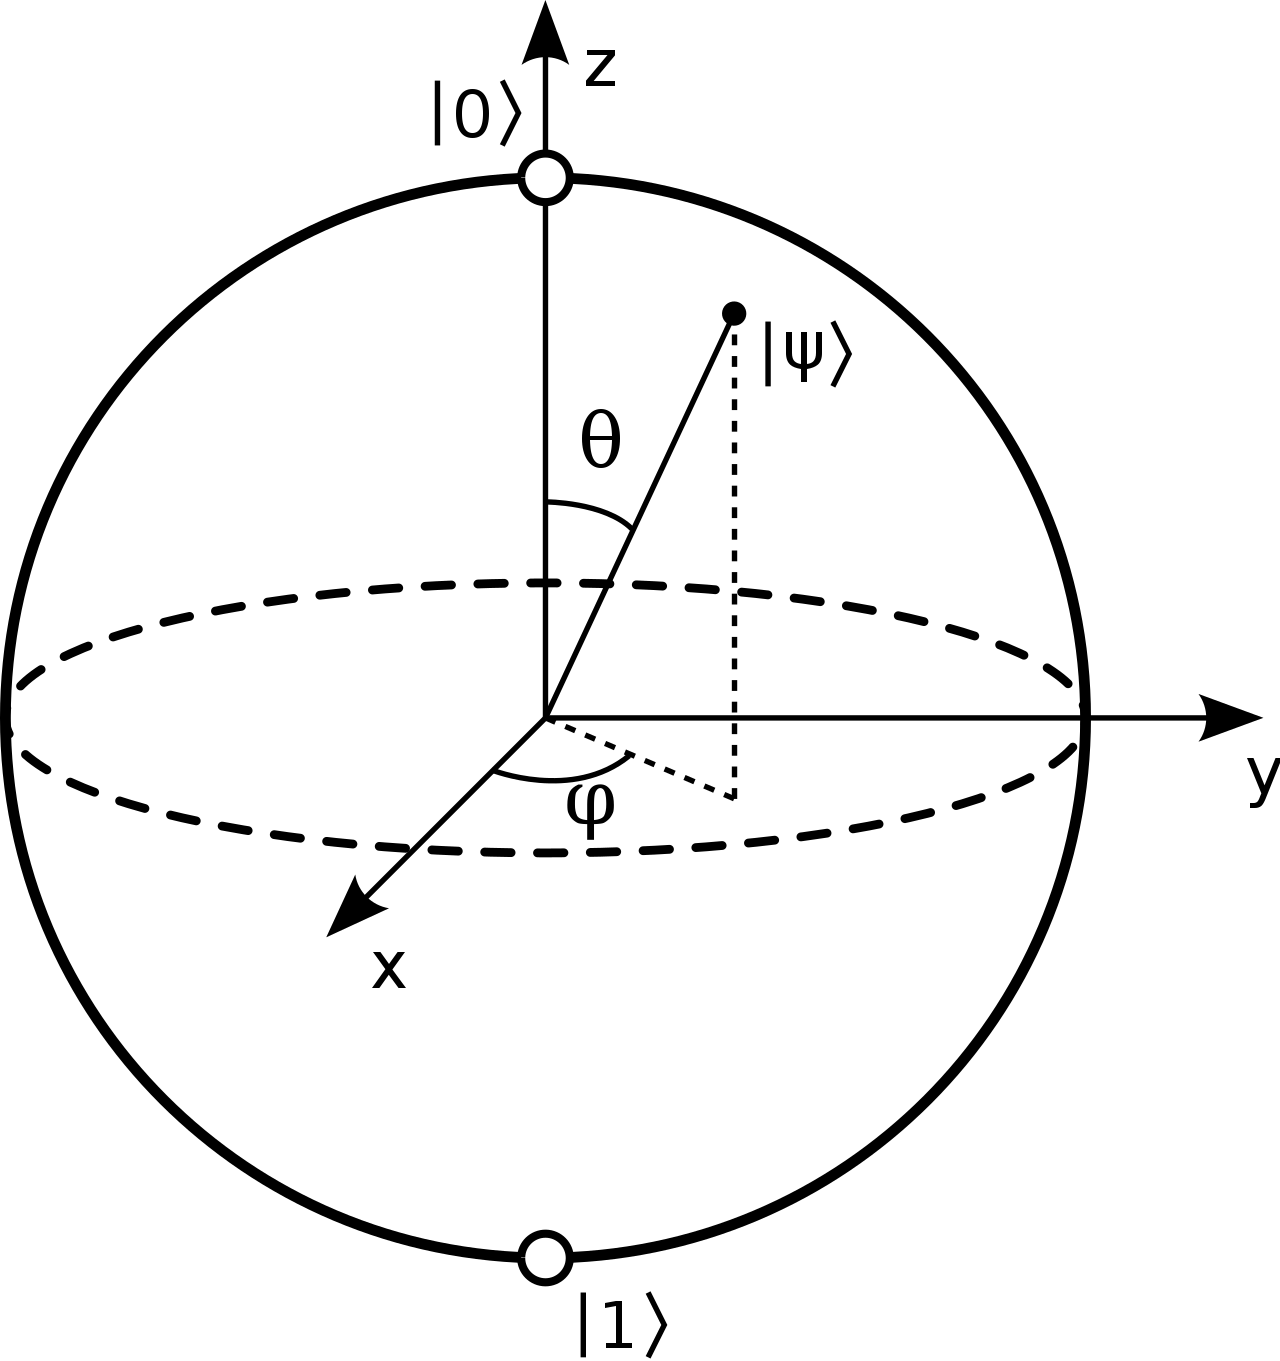
\includegraphics[width=0.4\textwidth]{fig/Bloch_sphere.svg}
  \caption{Representation of a Bloch sphere }%\cite{fig:Bloch-sphere}}
\end{figure}
%% Exkurs about the Hilbert fiber space for global phase factor and bloch sphere in higher dimensions

\chapter{Quantum Mechanics}

\section{Density operator}
Suppose we have a preparation of quantum states (such as sending photons through a polariser), that are not perfect with some impurity. Say that each possible \emph{pure} state $\ket{\Psi_1}, \cdots \ket{\Psi_K}$ with probabilities $P_1, \cdots P_K$. Suppose we measure an observable $A$ throught the operator $\hat A$ on this set of states, and we want to calculate the expectation value of this observable:
\begin{equation}
  A_{\textrm{av}} = \scalar{\hat A}_{\{P_k, \ket{\Psi_k}\}} = \sum{k=1}{K} P_k \scalar{\Psi_k \vert \hat A \vert \Psi_k} \label{eq:av-expectation-val}
\end{equation}
where this $K \in \N \cup \{\infty\}$ \emph{does not have to} be the same as dimension as the Hilbert space of the system. We can rewrite the equation \ref{eq:av-expectation-val} as:
\begin{align*}
 A_{\textrm{av}} & = \sum{k=1}{K} P_k \scalar{\Psi_k \vert \hat A \vert \Psi_k} \\
 & = \oldsum_k \oldsum_n P_k \scalar{\Psi_k \vert n} \scalar{n \vert \hat A \vert \Psi_k} \\
 & = \oldsum_k \oldsum_n P_k \scalar{n \vert \hat A \vert \Psi_k} \scalar{\Psi_k \vert n} \\
 & = \oldsum_k p_k \tr(\hat A \ket{\Psi_k} \bra{\Psi_k}) \\
 & = \tr\para{\hat A \oldsum_k p_k \ket{\Psi_k} \bra{\Psi_k}} \\
 & = \tr(\hat A \hat \rho)
\end{align*}
We define $\hat \rho := \oldsum_k p_k \ket{\Psi_k} \bra{\Psi_k}$ as the density operator representing the ensemble $\{p_k, \ket{\Psi_k}\}$

\subsection{Properties}
\begin{enumerate}[label = \alph*)]
  \item The density operator is a hermitian semi-definit operator: $\scalar{\hat \rho} \geq 0$. \\
  \begin{prf}
  \begin{equation*}
    \scalar{\Psi \vert \hat \rho \vert \Psi} = \oldsum_k p_k \abs{\scalar{\Psi \vert k}}^2 \geq 0 \forall \Psi \in \mathcal H
  \end{equation*}
  \end{prf}
  \item $\tr \hat \rho = 1$
  \item $\hat{\rho}^2 \leq \hat \rho$ and $\hat \rho^2 = \hat \rho \iff \hat \rho = \ket{\Psi_1}\bra{\Psi_1}$ called a pure state.
\end{enumerate}

\begin{example}
\textbf{Qubit density operator}: In diagonal (spectral) form, we can write the density operator as:
\begin{equation*}
  \hat \rho = p_0 \ket{\Psi_0}\bra{\Psi_0} + p_1 \ket{\Psi_1}\bra{\Psi_1}
\end{equation*}
where $\scalar{\Psi_0\vert\Psi_1} = 0$ and we can define the states $\Psi_0, \Psi_1$ as:
\begin{align*}
 \Psi_0 & = \cos\sfrac\theta 2 \ket{0} + \sin \sfrac\theta 2 e^{i\p} \ket{1} \\
 \Psi_1 & = - \sin \sfrac\theta 2 e^{-i\p}\ket{0} + \cos \sfrac\theta 2 \ket{1}
\end{align*}
with $p_0 + p_1 = 1$, so we can write these as: $p_0 = \frac{1 + r}{2}$, $p_1 = \frac{1 - r}{2}$, so we can write the density operator as:
\begin{equation}
  \hat \rho = \frac{1}{2} \para{\hat I + \v r \cdot \v \si}
\end{equation}
where $\v r(\sin\theta \cos\p, \sin\theta \sin\p, \cos\theta)$ is a $3D$-vector and $\si$ are the Pauli operators, and represent a point in the Bloch ball. For $r = 0$, the density operator is the identity operator and we have the maximal mixed state.
\end{example}

\section{Mixing theorem}
It was formulated by Hughstom et al. in PLA (1993)
\begin{tcolorbox}
  Consider $\hat \rho = \sum{k=1}{\dim(\mathcal H)} p_k \ket{e_k}\bra{e_k}$, where $\scalar{e_k \vert e_\ell} = \de_{k, \ell}$ and $\hat \eta = \sum{\ell = 1}{L} q_\ell \ket{\phi_\ell}\bra{\phi_\ell}$.
  Then $\hat \rho = \hat \eta$ iff there exists an unitary matrix $V \in \mat(\dim (\mathcal L) \times \dim(\mathcal L))$ such that
  \begin{equation}
  \sqrt{q_\ell} \ket{\phi_\ell} = \sum{k=1}{\dim \mathcal H} \sqrt{p_k} \ket{e_k} V_{kl} \forall l = 1, \cdots, \dim \mathcal H
  \end{equation}
\end{tcolorbox}



\section{Composite Systems}
In quantum mechanics we use tennsor products to describe states of composite systems. Assume me have systems a, b and c with bases, then the wave function of such a composite system can be written as:
\begin{equation}
  \ket{\Psi_{ABC}} = \oldsum_{k\ell m} a_{k\ell m} \ket{a_k} \otimes \ket{b_\ell} \otimes \ket{c_m}
\end{equation}
where the dimension of the Hilbert space is given by
\begin{equation}
  \dim \mathcal H_{ABC} = \dim \mathcal H_A \cdot \mathcal H_B \cdot \mathcal H_C
\end{equation}
is the number of combinations of basis vectors of the subsystems. As a notation we usually write
\begin{equation}
  \ket{a_k} \otimes \ket{b_\ell} \otimes \ket{c_m} \to \ket{a_k b_\ell c_m}
\end{equation}
As terminology: With $N$ subsystems, we mean a $N$ particle composite system.

Assume we have system of $N$ qubits, then the dimension of the composite system
\begin{equation*}
  \mathcal H_{2D}^{\otimes N} = \bigotimes_{i=1}^{N} \mathcal H_{2D}
\end{equation*}
with dimension
\begin{equation}
  \dim \mathcal H_{2D}^{\otimes N} = 2^N
\end{equation}
we can write the basis as binanry strings $x \in \{0, 1\}^N$ of length $N$ that generate the Hilbert space. A general wave function can then be written as
\begin{equation}
  \ket{\Psi_{N\textrm{-Qubit}}} = \sum{x=1}{2^N} c_x \ket{x}
\end{equation}


\subsection{Bipartite case}
In the bipartite case we set $N=2$ with subsystems A and B, an arbitrary pure state is described by
\begin{equation}
  \ket{\Psi^{AB}} = \sum{k=1}{n_A} \sum{\ell = 1}{n_B} a_{k\ell} \ket{k} \otimes \ket{\ell}
\end{equation}
with $n_i = \dim \mathcal H_i$.

\begin{theo}
It states, that:
\begin{equation}
  \ket{\Psi^{AB}} = \sum{m=1}{\min\{n_A, n_B\}} \sqrt{d_m} \ket{A_m} \otimes \ket{B_m}
\end{equation}
where $\ket{A_m} \in \mathcal H_A$ and $\scalar{A_m \vert A_{n}} = \de_{mn}$ for A and B and $\oldsum_m d_m = 1$.
\end{theo}

For the proof we need singular value decomposition: Assume $a \in \mat(n_A \times n_B)$ matrix. Then we can write this matrix $a$ as
\begin{equation*}
  a = U \cdot d \cdots V
\end{equation*}
where $U \in U(n_A)$, $V \in U(n_B)$ unitary matrices and $d$ a \say{diagonal} $n_A \times n_B$ matrix with the singular values $\sqrt{d_i}$ on the diagonal.
\begin{prf}

We view $a_{k\ell}$ as a $n_A \times n_B$ matrix. Then using singular value decomposition we get
\begin{equation*}
  a_{k\ell} = \sum{m=1}{\min\{n_A, n_B\}} U_{km} \sqrt{d_m} V{m\ell}
\end{equation*}
For a general bipartite wave function we get
\begin{align*}
  \ket{\Psi^{AB}} & = \sum{k=1}{n_A} \sum{\ell=1}{n_B} \sum{m=1}{\min\{n_A, n_B\}} U_{km} \sqrt{d_m} V{m\ell}\: \ket{k} \otimes \ket{\ell} \\
  & = \oldsum_{m} \sqrt{d_m} \oldsum_k U_{km} \ket{k} \otimes \oldsum_\ell V{m\ell} \ket{l} \\
  & = \sum{m=1}{\min\{n_A, n_B\}} \sqrt{d_m} \ket{A_m} \otimes \ket{B_m}
\end{align*}
It remains to prove, that orthonormality of the basis.
\begin{align*}
  \scalar{A_m \vert A_n} & = \sum{k, k'}{n_A} U_{km}^* U_{k'm} \scalar{k \vert k'} \\
  & = \sum{k=1}{n_A} U^\dagger_{mk} U_{kn} \\
  & = (U^\dagger U)_{m, n} = \de_{m,n}
\end{align*}
\end{prf}
There exists no generalisation to $N$ partite system. If it existsed it would take the form: $\Psi^{AB\cdots X} = \oldsum_m \sqrt{d_m} \ket{A_m} \cdots \ket{X_m}$


\begin{example}
Assume we have a 3-state qubit, we can write:
\begin{align*}
  \Psi^{ABC} & = \ket{000} + a \para{\ket{011} + \ket{101} + \ket{110}} \\
  & = \ket{+++} + \ket{---} = \ket{GHZ}
\end{align*}
where $\ket{\pm} = \ket{0} \pm \ket{1}$.

In comparason a state:
\begin{equation*}
  \ket{\Psi^{ABC}} = \ket{111} + a \para{\cdots}
\end{equation*}
that connot be decomposed into a Schmidt form. A similar state is
\begin{equation*}
  \ket{W} := \frac{1}{\sqrt{3}} \para{\ket{001} + \ket{010} + \ket{100}}
\end{equation*}
that has no Schmidt decomposition.
\end{example}

\section{Reduced denisty operator, partial trace}

Assume we have a bipartite system with state $\ket{\Psi^{AB}}$. What does it mean to only have accoess to onu of the two subsystems, say A? Vhat does it do operationally. Suppose we measure observable $O_A$ an A, then using Schmidt decomposition
\begin{align*}
  \scalar{\hat O_A}_{\Psi^{AB}} & = \scalar{\Psi^{AB} \vert \hat O_A \otimes \hat I_B \vert \Psi^{AB}} \\
  & = \oldsum_{k\ell} \sqrt{d_k} \sqrt{d_\ell} \scalar{A_k \vert \hat O_A \vert A_\ell} \scalar{B_k \vert \hat I \vert B_\ell} \\
  & = \oldsum_{k} d_k \scalar{A_k \vert \hat O_A \vert A_k} \\
  & = \tr\para{O_A \oldsum_k d_k \ket{A_k} \bra{A_k}} \\
  & = \tr\para{O_A \rho_B}
\end{align*}
where $\rho_A$ is the reduced density operator in spectral form. A reduced density operator can be computed as a partial trace:
\begin{equation}
  \rho_A = \tr_A \ket{\Psi^{AB}} \bra{\Psi^{AB}} = \oldsum_m \scalar{B_m \vert \Psi^{AB}} \scalar{\Psi^{AB} \vert B_m}
\end{equation}


\section{Completely positive maps (quantum channels)}
Within the space of all possible states (Bloch sphere for a single qubit), we can have maps between different quantum states. If we restrict ourselves to only using unitary transformation, that pure states can only stay pure states (called \emph{closed system}) whereas completely positive maps that can transform a system more generally.

\begin{defi}
A completely positive map (CMP) $\rho \to \mathcal E(\rho) \geq 0$ satisfies:
\begin{enumerate}[label = (\alph*)]
  \item $\tr[\mathcal E(\rho)]$ is the probability that $\mathcal E$ happens:
  \begin{subequations}
  \begin{equation}
    \Longrightarrow 0 \leq \tr[\mathcal E(\rho)] \leq 1,
  \end{equation}
  with $\tr[\mathcal E(\rho)] = 1$ if the CPM is a completely positive trance perserving (CPTP) map.
  \item A CMP should be linear, so that: $\mathcal E \para{\oldsum_k p_k \rho_k} = \oldsum_k p_k \mathcal E(\rho_k)$.
  \item Let $A, B$ be positive semi-definit operator, then the following inequality should hold
  \begin{equation}
    \mathcal E(A) \geq 0 \qquad \text{(positivity)}
  \end{equation}
  and, if $B$ is an operator that acts on a langer Hilbert space, then
  \begin{equation}
    \mathcal E \otimes \mathcal I(B) \geq 0
  \end{equation}
  for \emph{any} extension of the system (complete positivity). This conditions guaranties that remote systems cannot influence the physical nature of $\mathcal E$
  \end{subequations}
\end{enumerate}
\end{defi}
\begin{defi}
Transposition:
\begin{equation}
\para{\ket{A} \bra{A^\perp}}^T =  \ket{A^\perp}\bra{A}
\end{equation}
(partial transpostion)
\end{defi}

\begin{example}
We have the state:
\begin{align*}
  \ket{\Psi^{AB}} & = \frac{1}{\sqrt{2}} \para{\ket{01} - \ket{20}} \quad\to\quad \rho_{AB}^{T_A} = \ket{\Psi^{AB}} \bra{\Psi^AB}^{T_A} \\
  & = \frac{1}{2} \para{\ket{01} - \ket{10}}\para{\bra{01} - \bra{10}}^{T_A} \\
  & = \frac{1}{2} \para{\ket{01}\bra{01} - \ket{01}\bra{10} - \ket{10}\bra{01} + \ket{10}\bra{10}}^{T_A} \\
  & = \frac{1}{2} \para{\ket{0}\bra{0} \otimes \ket{1}\bra{1} - \ket{0}\bra{1} \otimes \ket{1} \bra{0} - \ket{0} \bra{1} \otimes \ket{0} \bra{1} + \ket{1}\bra{1} \otimes\ket{0} \bra{0}} \\
  & =
  \begin{pmatrix}
    0 & 0 & 0 & \sfrac{1}{2} \\
    0 & \sfrac{1}{2} & 0 & \\
    0 & 0 & \sfrac{1}{2} & 0 \\
    \sfrac{1}{2} & 0 & 0 & 0
  \end{pmatrix}
\end{align*}
with eigenvalues $\left\{\frac{1}{2}, \frac{1}{2}, \frac{1}{2}, -\frac{1}{2}\right\}$
\end{example}


\begin{theo}
    $\mathcal E$ is a CPM $\iff \exists \{E_k\}$ such that
    \begin{equation}
      \oldsum_k E_k^\dagger E_k \leq \hat 1
    \end{equation}
    where the equality is given for CPTP maps in terms of which
    \begin{equation}
      \mathcal E(\rho) = \oldsum_k E_k \rho E_k^\dagger
    \end{equation}
    called the Kraus representation or operator sum representation and the $E_k$ are called Kraus operators.
\end{theo}

\begin{example}
\say{Decay of an atom}
Let $\ket{e}$ be the excited state of a atom and $\ket{g}$ be its ground state. Then the Kraus operators are
\begin{equation*}
  \begin{cases}
    E_0 & = \ket{g}\bra{g} + \sqrt{1 - \gamma} \ket{e} \bra{e} \\
    E_1 & = \sqrt{\gamma} \ket{g}\bra{e}
  \end{cases}
\end{equation*}
with $\gamma \in [0, 1]$. So
\begin{align*}
  \rho & \to E_0 \rho E_0^\dagger + E_1 \rho E_1^\dagger \\
  & = \para{\ket{g} \bra{g} + \sqrt{1 - \gamma} \ket{e} \bra{e}} \rho \para{\ket{g} \bra{g} + \sqrt{1 - \gamma} \ket{e} \bra{e}} +   \para{\gamma \ket{g}\bra{e}} \rho \ket{e}\bra{g} \\
  & \underset{\gamma \shortto 1}{\to} \ket{g}\scalar{g \vert \rho \vert g} \bra{rho} + \ket{g}\scalar{e \vert \rho \vert e} \bra{rho} \\
  & = \ket{g}\bra{g} \underbrace{\para{\scalar{g \vert \rho \vert g} + \scalar{e \vert \rho \vert e}}}_{\tr \rho = 1} \\
  & = \ket{g}\bra{g}
\end{align*}
a decay with $\gamma = 1 - e^{-\lambda t}$.
\end{example}

\subsection{Stine spring dilation}
Assume we have a system $s$ in an environement $e$ and we want to determine the effect of the environement on the system with the time evolution operator $U_{se}$, then we can decompose the state:
\begin{equation}
  \rho_{se} = \rho \otimes \ket{e_0} \bra{e_0}
\end{equation}
With a unitary map:
\begin{equation*}
  \rho_{se} \mapsto U_{se} \rho \otimes \ket{e_0} \bra{e_0} U_{se}^\dagger
\end{equation*}
The map of the system gives us:
\begin{align*}
  \rho & \mapsto \tr_e\para{U_{se} \rho_{se} U_{se}^\dagger}
  & = \sum{n=0}{\dim \mathcal H_e - 1} \scalar{e_n \vert U_{se} \rho \otimes \vert e_0} \scalar{e_0 \vert U_{se}^\dagger \vert e_n} \\
  & = \oldsum_n \scalar{e_n \vert U_{se} \vert e_0} \rho \scalar{e_0 \vert U_{se}^\dagger \vert e_n} \\
  & = \oldsum_n E_n \rho E_n^\dagger
\end{align*}
To prove that $\para{\scalar{e_n \vert U_{se} \vert e_0}}^\dagger = \scalar{e_n \vert U_{se}^\dagger \vert e_0}$ use:
\begin{equation*}
  \oldsum_{k\ell,pq} \ket{s_k} \ket{s_\ell} (U_{se})_{k\ell, pq} \bra{s_q} \bra{p}
\end{equation*}
This is a CPTP map:
\begin{align*}
  \oldsum_n E_n^\dagger E_n & = \oldsum_n \para{\scalar{e_n \vert U_{se} \vert e_0}}^\dagger \scalar{e_n \vert U_{se} \vert e_0} \\
  & = \oldsum_n \scalar{e_0 \vert U_{se}^\dagger \vert e_n} \scalar{e_n \vert U_{se} \vert e_0} \\
  & = \scalar{e_0 \vert U_{se}^\dagger U_{se} \vert e_0} \\
  & = \hat I_s \scalar{e_0 \vert \hat I_e \vert e_0} = \hat I_s
\end{align*}
One can use Stinespring dilation to prove that the Kraus representation is not unique. Using a basis transformation: $\ket{e_n} \mapsto \ket{f_n} = \oldsum_m \ket{e_m} U^\dagger_{mn}$ with a unitary basis transformation $U$. As $U$ only is unitary transformation should not affect the map. Kraus operators $\{F_n = \scalar{f_n \vert U_{se} \vert e_0}\}$ define the same map as $\{E_n = \scalar{e_n \vert U_{se} \vert e_0}\}$, one finds
\begin{equation*}
  F_n = \oldsum_m U_{mn} E_m
\end{equation*}

\section{Application of the CPM formalism:}
\subsection{Measurement}
A generalized measurement is a CPTP map with the following interpretation:
\begin{enumerate}[label = (\roman*)]
  \item Each measurement outcome $m_k$ is associated with a Kraus operator $E_k$.
  \item The \textbf{Born rule}: the probability $P(m_k \vert \rho)$ is given by:
  \begin{equation}
    P(m_k \vert \rho) = \tr(E_k^\dagger E_k \rho)
  \end{equation}
  \item Update the probability distribution (i.e. the state) usnig the following rule:
  \begin{equation}
    \rho \underset{m_k}{\to} E_k \rho E_k^\dagger
  \end{equation}
\end{enumerate}
The special case called von Neumann or projective measurment we have $E_k = \ket{k}\bra{k}$ and the measurement with probability yields:
\begin{align*}
  P(m_k \vert \rho) & = \tr(\ket{k}\bra{k} \ket{k}\bra{k} \rho) \\
  & = \tr(\ket{k} \bra{k} \rho) \\
  & = \scalar{k \vert \rho \vert k}
\end{align*}
if $\rho = \ket{\Psi} \bra{\Psi}$, then:
\begin{align*}
  \Longrightarrow P(m_k \vert \rho) & = \scalar{k \vert \Psi} \scalar{\Psi \vert k} \\
  & = \abs{\scalar{k \vert \Psi}}^2
\end{align*}
\begin{note}
  The sum of the probabilty of all outcomes:
  \begin{align*}
    \oldsum_k P(m_k \vert \rho) & = \oldsum_k \tr(E_k^\dagger E_k \rho) \\
    & = \tr\para{\oldsum_k \underbrace{E_k^k E_k}_{\hat I} \rho} \\
    & = \tr \rho = 1
  \end{align*}
\end{note}
\begin{notation}
  We define $\{\Pi_k := E_k^\dagger E_k \}$ as a positive operator valued measure (POVM).
\end{notation}

\begin{theo}
  Non-orthogonal states can not be distinguished in a general measurement
\end{theo}

\begin{prf}
  Assume $\ket{\Phi}$ and $\ket{\Psi}$ are non-orthogonal and \emph{can} be distinguished. If this is possible then there exists $\Pi_1$ and $P_2$ such that $\scalar{\Psi \vert \Pi_1 \vert \Psi} = 1$ and $\scalar{\Phi \vert \Pi_2 \vert \Phi} = 1$.
  Because probabilities must add up to $1$, we must have $\scalar{\Psi \vert \Pi_2 \vert \Psi} = 0$ where $\Pi_k \geq 0$, so $\sqrt{\Pi_k} \geq 0$. We get:
  \begin{equation*}
    0 = \scalar{\Psi \vert \Pi_2 \vert \Psi} = \norm{\sqrt{\Pi_2} \ket{\Psi}}^2
  \end{equation*}
  so $\sqrt{\Pi_2} \ket{\Psi} = 0$ ($0$-vector). \\
  We can write $\ket{\Phi} = a \ket{\Psi^\perp} + b \ket{\Psi}$ where $b \neq 0$ by assumption. This implies also that $\abs{a}^2 + \abs{b}^2 = 1$, so $\abs{a}^2 < 1$. Thus
  \begin{align*}
    \sqrt{\Pi_2} \ket{\Phi} & = a \sqrt{\Pi_2} \ket{\Psi^\perp} + b \sqrt{\Pi_2} \ket{\Psi} \\
    & = a \sqrt{\Pi_2} \ket{\Psi^\perp}
  \end{align*}
  So
  \begin{equation*}
    \begin{cases}
      \norm{\sqrt{\Pi_2} \ket{\Psi^\perp}} & = \scalar{\Phi \vert \Pi_2 \vert \Phi} = 1 \\
      \norm{\sqrt{\Pi_2} \ket{\Psi^\perp}} & = \abs{a}^2 \scalar{\Psi^\perp \vert \Pi_2 \vert \Psi^2} \leq \abs{a}^2 < 1
    \end{cases}
  \end{equation*}
\end{prf}

\subsection{Lindblad equation}
So far we have only been looking at discreet maps through CPMs. How would the dynamics of an open system be described, from a time $\rho_0$ to a time $T\; \rho_T$. We can model such case throught a series of small CPMs for timesteps $\Delta t \to 0$, where the environemental state is measured at each timesteps $t_i$, and the system always can be described as a product state. \\
We can map the density operator as a sequence of CPM (Markonvian approximation)
\begin{align*}
  \rho & \mapsto \mathcal E_{k \de t, (k-1)\de t} \circ \cdots \circ \mathcal E_{2\de t, \de t} \circ \mathcal E_{\de t, 0} (\rho_0)
\end{align*}
We do the simplifying assumption, that $\mathcal E_{t + \de t, \de t} \equiv \mathcal E_{\de t}$ (which implies that the Hamiltonian of the system is time independent). We consider the map
\begin{align*}
\rho_t \mapsto \rho_{t + \de t} & = \oldsum_k E_k(\de t) \rho_t E_k^\dagger(\de t) \\
& = \mathcal E_{\de t}(\rho_t) \\
\mathcal E_{\de t} & \underset{\de t \shortto 0}{\to} \mathcal I
\end{align*}
with $\mathcal I$ being the identity map. \\
This allows us to make an ansatz:
\begin{equation*}
  E_0 (\de t) = 1 - i(H - iG) \de t
\end{equation*}
With $H$ and $G$ hermitian operators.
\begin{equation*}
  E_{k>0} (\de t) = \sqrt{\de t} L_k
\end{equation*}
We assume that $\mathcal E_{\de t}$ is a CPTP since we do not exctact information of the system during the evolution, in other words $\tr \rho_t = 1$ for all $t$. This implies for our ansatz:
\begin{align*}
  \hat I & = \oldsum_k E_k^\dagger (\de t) E_k (\de t) \\
  & = E_0^\dagger (\de t) E_0(\de t) + \sum{k=0}{} E_k^\dagger (\de t) E_k(\de t) \\
  & = \hat I + 2 G \de t + \de t \sum{k=1}{} L_k^\dagger L_k + O(\de t^2)
\end{align*}
So we get:
\begin{equation}
  G = \frac{1}{2} \sum{k=1}{} L_k^\dagger L_k
\end{equation}
This gives us the Lindblad equation:
\begin{align}
  \frac{\rho_{t + \de t} - \rho_t}{\de t} & = - i [H, \rho_t] + \oldsum_k \para{L_k \rho L_k^\dagger - \frac{1}{2} \{L_k^\dagger L_k, \rho\}} \nonumber\\
  \de t \to 0 \Longrightarrow \dot{\rho}_t & = - i [H, \rho_t] + \oldsum_k \para{L_k \rho_t L_k^\dagger - \frac{1}{2} \{L_k^\dagger L_k, \rho_t\}}
\end{align}
where $\{A, B\} = AB + BA$ is the anticommutator, and $H$ should be interpreted as the Hamiltonian, thus the first term of the equation is called the \say{Schrödinger term}, the $L_k$ are called Lindblad operators and the anticommutator term give non hermitian dynamics.

\begin{example}
Assume a qubit system with $L = \sqrt{\gamma} \si_z$ with Hamiltonian $H = \omega \si_z$, would give a density operator:
\begin{equation*}
  \rho_t = \frac{1}{2} (\hat I + \v r_t \cdot \v \si)
\end{equation*}
with the solution in the rotating frame.
\begin{align*}
  \dot{\v r} & = - 2 \gamma (x_t, y_t, 0) \\
  \v r & = (x_0 e^{-2 \gamma t}, y_0 e^{-2 \gamma t}, z_0)
\end{align*}
which for $t \to \infty$, we end up with a state lying on the $z$-axis, and the exponential term in the $x$ and $y$ coordinates are called decoherence terms.
\end{example}


\chapter{Quantum entanglement and cloning}

\section{Quantum entanglement}
In the beginning, we only talk about the bipartite case. We can divide our system into two subsystems.
\begin{defi}
A state $\ket{\Psi_{AB}} \in \mathcal H_A \otimes \mathcal H_B$ is entangled iff it cannot be written as a product state $\ket{\phi_A}\otimes\ket{phi_B}$
\end{defi}
\begin{example}
  Given a 2 qubit system
  \begin{equation*}
    \ket{\Psi_{AB}} = a \ket{00} + b \ket{01} + c \ket{10} + d \ket{11}
  \end{equation*}
  with $a,b,c,d \in \C$ and $\scalar{\Psi_{AB} \vert \Psi_{AB}} = 1$. How do determine if this state can be written as a product state.
  \begin{itemize}
    \item We can put this into Schmidt form, so that:
    \begin{equation*}
      \ket{\Psi_{AB}} = \sum{k=1}{2}\sqrt{d_k} \ket{A_k} \otimes \ket{B_k}
    \end{equation*}
    then, $\ket{\Psi_{AB}}$ is entangled iff $d_1\cdot d_2 \neq 0$.
    \item We can compute the reduced density operator $\rho_A = \tr_B \ket{\Psi_{AB}}\bra{\Psi_{AB}} = \sum{k=1}{2} d_k \ket{A_k} \bra{A_k}$, then if $d_1 \cdot d_2 \neq 0$ implies $\rho_A$ is a non-pure stare. Thus, if $\rho_A$ is non-pure, then $\ket{\Psi_{AB}}$ is mixed and vice versa.
    \item In the this example, there is an easy way to deterime entanglement. Iff $ad-bc \neq 0$, then $\ket{\Psi_{AB}}$ is entangled.
  \end{itemize}
\end{example}

Let us consider a mixed state with $\rho_{AB} \geq 0$ and $\tr \rho_{AB} = 1$.
\begin{tcolorbox}
  \begin{equation}
    \rho_{AB} = \rho_A \otimes \rho_B \quad\to\quad \tr_B \rho_{AB} = \rho_A \tr \rho_B = \rho_A
  \end{equation}
\end{tcolorbox}
How do we determine entanglement for $\rho_{AB}$?

\begin{idea}
  Suppose we have many copies of $\rho_A \otimes \rho_B$ and suppose that Alice and Bob can perform \say{coordinated} local operations $\{p_k, \mathcal E_k \otimes \mathcal F_k\}$ leading to:
  \begin{align*}
    \rho_{AB} & = \oldsum_k p_k \mathcal E_k \otimes \mathcal F_k (\rho_A \otimes \rho_B) \\
    & = \oldsum_k p_k \mathcal E_k(\rho_A) \otimes \mathcal F_k(\rho_B) \\
    & = \oldsum_k p_k \rho_A^k \otimes \rho_B^k
  \end{align*}
  Since we only use local operations and classical communication (LOCC) starting from a product state, the output will \emph{not} be entangled such a state is called separable.
\end{idea}

\begin{defi}
    A state $\rho_{AB}$ is entangled iff it \emph{cannot} be written in the form $\oldsum_k p_k \rho_A^k \otimes \rho_B^k$.
\end{defi}

\section{Entanglement detection}
We are given a state $\rho_{AB}$, how do we determine if it is entangled or not?
\begin{theo}[Horodedu family : Phy. lett A (1996)]

  $\rho_{AB}$ is separable $\iff$ for every \say{positive} map $\mathcal A$ on one of the subsystems $\mathcal A \otimes I_B (\rho_{AB}) \geq 0$.
  \end{theo}
\begin{itemize}
  \item \emph{Useful test}: (PPT = positive partial transposition) \\
  \begin{equation}
    \rho^{AB}\: \textrm{is seperable} \Longrightarrow \para{\rho^{AB}}^{T_A} \geq 0
  \end{equation}
  The implication to the other side only holds for $2 \otimes 2$ or $2 \otimes 3$ systems.
\end{itemize}

\section{Quantifying entanglement}
\begin{defi}
  We can quantifying entanglement by using a measurment function
  \begin{equation*}
    \mu:  \mathcal H_A \otimes \mathcal H_B \to  \R \; : \: \rho^{AB} \mapsto \mu(\rho^{AB})
  \end{equation*}
  This measurment function should furfill:
  \begin{itemize}
    \item $\mu \geq 0$
    \item $\mu = 0$ for separable states
    \item $\mu$ is be non-increasing under LOCC
    \item $\mu$ is invariant under local unitary operations.
  \end{itemize}
\end{defi}
There are \emph{two} measures:
\begin{enumerate}[label=(\alph*)]
  \item \emph{Negativity}: Based on PPT:
  \begin{align*}
    \mathcal N_e (\rho^{AB}) = \frac{\tr\abs{\para{\rho^{AB}}^{T_A}} - 1}{2} = \frac{\norm{\para{\rho^{AB}}^{T_A}} - 1}{2}
  \end{align*}
  where $\norm{\rho} := \tr\sqrt{A^\dagger A}$
  \begin{example}
    We look at the state $\ket{\Psi^{AB}} = \frac{1}{\sqrt{2}} \para{\ket{01} - \ket{10}}$ where the eigenvalues of $\para{\ket{\Psi^{AB}} \bra{\Psi^{AB}}}^{T_A}$ are $\frac{1}{2}$, $\frac{1}{2}$,  $\frac{1}{2}$, $-\frac{1}{2}$. so the negativity is non-zero.
  \end{example}
  \item \emph{Concurrence}: Only works for $2 \times 2$ systems from its definition. \\
  Based on the univeral flip: $\Theta(\alpha \ket{0} + \beta\ket{1}) = - \beta^*\ket{0} + \alpha^*\ket{1}$, that is orthogonal to the initial state (such an aperation cannot be made, because we cannot make comlped conjugation). \\
  A pure state of two qubits written in Schmidt decomposition:
  \begin{align*}
    \ket{\Psi_{AB}} & = \sum{k=0}{1} \sqrt{d_k} \ket{A_k} \otimes \ket{B_k} \\
    & = \sqrt{d_k} \ket{A_0} \otimes \ket{B_0} + \sqrt{d_1} \ket{A_1} \otimes \ket{B_1} \overset{\say{\Theta_A\otimes \Theta_B}}{\to} \\
    & \to \sqrt{d_0} \ket{A_1} \otimes\ket{B_1} + \sqrt{d_1} \ket{A_0} \otimes \ket{B_0} =: \ket{\tilde \Psi_{AB}} \\
    & \Longrightarrow \abs{\scalar{\tilde \Psi_{AB} \vert \Psi_{AB}}} = 2 \sqrt{d_0 d_1} = 2 \sqrt{d_0 (1 - d_0)} \leq 1
  \end{align*}
  with equality if $d_0 = \frac{1}{2}$. \\
  The concurrence $C(\Psi_{AB})$
\end{enumerate}


\subsection{Generalization to mixed states (Wootters, PRL 1998)}
Given a state $\rho_{AB}$
\begin{itemize}
  \item Qubit flip: $\rho_{AB} \mapsto \tilde \rho_{AB} = \si_y \otimes \si_y \mathcal K(\rho_{AB}) \si_y \otimes\si_y$ where $\mathcal K$ is the comlpex conjugation with regard to the product basis $\ket{00}, \cdots, \ket{11}$.
  \item Compute the eigenvalues $\lambda_k$ of $\rho_{AB}\tilde \rho_{AB}$.
  \item We compute: $\max\{0, \sqrt{\lambda_1} - \sqrt{\lambda_2} - \sqrt{\lambda_3} - \sqrt{\lambda_4}\} = C(\rho_{AB})$, where $\lambda_1$ is the largest eigenvalue. 
\end{itemize}



\appendix
\chapter{Exercices}
\section{Qubit}

\section{Quantum ensemble: Density operator}

\section{Composite system}

\section{Completely positive maps}
18. \begin{enumerate}[label = (\alph*)]
  \item The phase damping completely positive map: $\mathcal E(\rho) = (1-p)\rho + p \si_z \rho \si_z$ for $p \in [0, 1]$. The Kraus operators are
  \begin{equation*}
    \begin{cases}
      E_0 & = \sqrt{1 - p} \hat I \\
      E_1 & = \sqrt{p} \hat \si_z
    \end{cases}
  \end{equation*}
  \item The bit flip map $\mathcal E(\rho) = (1-p)\rho + p \si_x \rho\si_x$ for $p\in [0, 1]$. The Kraus operators are
  \begin{equation*}
    \begin{cases}
      E_0 & = \sqrt{1 - p} \hat I \\
      E_1 & = \sqrt{p} \hat \si_x
    \end{cases}
  \end{equation*}
  \item The phase shape and bit shift map $\mathcal E(\rho) = (1-p)\rho + p \si_y \rho\si_y$ for $p\in [0, 1]$. The Kraus operators are
  \begin{equation*}
    \begin{cases}
      E_0 & = \sqrt{1 - p} \hat I \\
      E_1 & = \sqrt{p} \hat \si_y
    \end{cases}
  \end{equation*}
\end{enumerate}
22. Consider a two lever atom with ground state $\ket{g}$ and excited state $\ket{e}$. The atom is placed in a cavity, which includes decay of an atom modeled by the unitary transformation
\begin{align*}
  \ket{e} \otimes \ket{n} & \mapsto \sqrt{1 - p} \ket{e} \otimes\ket{n} + \sqrt{p} \ket{g} \otimes \ket{n+1}\\
  \ket{g} \otimes \ket{n} & \mapsto \ket{g} \otimes \ket{n}
\end{align*}
where $\ket{n}$ and $\ket{n+1}$ are the states of the quantizised field corresponding to the $n$ and $n+1$ photons in the cavity. Suppose the atom+cavity field start in the pure states
\begin{equation*}
  \ket{\Psi} = \para{\cos \sfrac \theta 2 \ket{g} + \sin \sfrac \theta 2 \ket{g}} \otimes \ket{n}
\end{equation*}
and undergoes a decay. Compute the average number of photons in the cavity as a function of the decay probability $p$. \\
The expectation value is $\scalar{N} = \scalar{a^\dagger a} = \tr(\mathcal E(\rho_{\gamma}) N)$. The density of the composite system is:
\begin{equation}
  \rho_{a\gamma} = \ket{\Psi}\bra{\Psi} = \ket{\Psi_0} \bra{\Psi_0} \otimes \ket{n}\bra{n}
\end{equation}
Now appling the positivy map and calculate the partial trace.
\begin{align*}
  \mathcal E(\rho_{a\gamma} & = \left[\mathcal E (\ket{\Psi})\right]\left[\mathcal E (\ket{\Psi})\right]^\dagger \\
  & = \tr_a(\mathcal E(\rho_{a\gamma})) = ...
\end{align*}
An alternative: From the lecture, we know, that a composite system evolves as $\rho_{se} \to U_{se} \rho_{se} U_{se}^\dagger$, then the system has a Kraus decomposition
\begin{equation*}
  \rho \to \oldsum E_n \rho E_n^\dagger
\end{equation*}
where $E_n = \scalar{E_n \vert U_{se} \vert E_0}$ with $E_n$ an orthogonal basis for the environement. On out atom system, we need to determine the basis for the composite system $\{\ket{g} \ket{0}, \ket{g}\ket{0}, \cdots, \ket{g} \ket{n}, \cdots, \ket{e}\ket{0}, \cdots \ket{e}\ket{n}, \cdots\}$.
As a matrix, the time evolution operator looks like:
\begin{equation*}
  U =
  \begin{pmatrix}
    1 &&&&& 0 &&&& \\
    & 1 & &&& \sqrt{p} & \ddots \\
    && \ddots &&&& \ddots \\
    &&& 1 &&&& 0 \\
    &&&& \ddots &&& \sqrt{p} & \ddots \\
    &&&&& \sqrt{1 - p} &&& \ddots \\
    &&&&&& \ddots  \\
    &&&&&&& \sqrt{1 - p} \\
    &&&&&&&& \ddots
  \end{pmatrix} =
  \begin{pmatrix}
    I & B \\
    0 & C
  \end{pmatrix}
\end{equation*}
We can calculate the Kraus coeffitions:
\begin{equation*}
  \begin{cases}
    E_g & = \scalar{g \vert U_{ac} \vert \Psi_0} \\
    E_e & = \scalar{e \vert U_{ac} \vert \Psi_0}
  \end{cases}
\end{equation*}
with $\ket{\Phi_0} = \cos\sfrac\theta 2 \ket{g} + \sin \sfrac\theta 2 \ket{e}$ and get:
\begin{align*}
  E_g & = \cos\sfrac\theta 2 \scalar{g \vert U_{ac} \vert g} + \sin\sfrac\theta 2 \scalar{g \vert U_{ac} \vert e} \\
  & = \cos\sfrac\theta 2 I + \sin \sfrac\theta 2 B \\
  E_e & = \cos \sfrac\theta 2 \scalar{e \vert U_{ac} \vert g} + \sin\sfrac\theta 2 \scalar{e \vert U_{ac} \vert e} \\
  & = \sin\sfrac\theta 2 C
\end{align*}
So we get:
\begin{align*}
  \mathcal E(\rho) & = \mathcal E(\ket{n}\bra{n}) \\
  & = E_g \ket{n}\bra{n} E_g^\dagger + E_e \ket{n}\bra{n} E_e^\dagger \\
  & = \cos^2 \sfrac \theta 2 \ket{n}\bra{n} + \cos\sfrac \theta 2\sin\sfrac \theta 2\para{\ket{n}\bra{n} B^\dagger + B \ket{n}\bra{n}} \\
  & \phantom{=} + \sin^2\sfrac \theta 2 B \ket{n}\bra{n} B^\dagger + \sin^2\sfrac \theta 2\sin C \ket{n}\bra{n} C^\dagger \\
  & = \left[\cos^2\sfrac \theta 2 + (1-p) \sin^2\sfrac \theta 2\right] \ket{n}\bra{n} + p \sin^2 \sfrac \theta 2 \ket{n+1} \bra{n+1} \\
  & \phantom{=} + \sqrt{p} \sin\sfrac \theta 2\cos\sfrac \theta 2 \left[ \ket{n} \bra{n+1} + \ket{n+1}\bra{n}\right] \\
\end{align*}
We can now calculate the expectation value of $N$ with $N \ket{n} = a^\dagger a \ket{n} = n$
\begin{align*}
  \scalar{N} & = \tr(\mathcal E(\rho_c) N) \\
  & = n \left[\cos^2 \sfrac \theta 2 + (1 - p)\sin^2\sfrac \theta 2\right] + (n+1) p \sin^2 \sfrac \theta 2 \\
  & = n + p \sin^2 \sfrac \theta 2
\end{align*}


\section{Lindblad equation}
26. Let $H$ be the Hamiltonian:
\begin{equation*}
  H = \oldsum E_k \ket{\Phi_k}\bra{\Phi_k}
\end{equation*}
with an error $L = \sqrt{\gamma}H$. Let $\rho(t)$ be the state of the system at time $t$, then:
\begin{equation*}
  \dot{\rho}(t) = - i [H, \rho] + \oldsum \para{L_n \rho L_n^\dagger - \frac{1}{2}\{L_n^\dagger L_n, \rho\}}
\end{equation*}
We want to show, that it reduced to
\begin{equation*}
  \dot{\rho}(t) = - [H, \rho] - \frac{\gamma}{2} [H, [H, \rho]]
\end{equation*}
We only need to show, that:
\begin{align*}
  L \rho L^\dagger - \frac{1}{2} \{LL^\dagger, \rho\} & = \gamma \para{H \rho H - \frac{1}{2} (H^2\rho + \rho H^2)} \\
  -\gamma [H, [H, \rho]] & = -\gamma \para{H, H \rho - \rho H} \\
  & = -\gamma \para{H^2 \rho - H \rho H - H\rho H + \rho H^2} \\
  & = \frac{\gamma}{2} \para{ H \rho H - \frac{1}{2}(H^2 \rho + H^2 \rho)}
\end{align*}
This is the damping equation used in magnetism.
We can write the density operator as
\begin{equation*}
   \rho = \oldsum_{\ell k} = \rho_{k\ell}(t) \ket{\Phi_k} \bra{\Phi_\ell}
\end{equation*}
that, because of linearity, we only need to solve them for one of the $\rho_{k\ell}$
\begin{align*}
  \dot{\rho}_{k\ell}(t) & = - \rho_{k\ell} [H, \ket{\Phi_k}\bra{\Phi_\ell}] - \frac{\gamma}{2} \rho_{k\ell} [H, [H, \ket{\Phi_k}\bra{\Phi_\ell}]] \\
  % & = \rho_{k\ell}(t) \para{-i \para{H \ket{\Phi_k}\bra{\Phi_\ell} - \ket{\Phi_k}\bra{\Phi_\ell} H} - \frac{\gamma}{2}}   \\
  & = \rho_{k\ell}(t) \para{-i (E_k - E_\ell) - \frac{\gamma}{2} (E_k - E_\ell)^2} \ket{\Phi_k}\bra{\Phi_\ell}
\end{align*}
And we get
\begin{equation*}
  \rho_{k\ell} (t) e^{t(-i(E_k - E_\ell))} e^{-\frac{\gamma t}{2}(E_k - E_\ell)^2}
\end{equation*}
For $\gamma t \shortto \infty$, $\rho_{k\ell}$ goes to $0$.


\section{Measurements}

\section{Quantum Entanglement}

\section{Detecting quantum entanglement}

\section{Quantifying quantum entanglement}

\section{Quantum teleportation}

\section{Bell's inequality}

\section{Quantum copying}

\section{von Neumann and relative entropy}


\end{document}
